\documentclass[10pt,letterpaper]{article}
\renewcommand{\rmdefault}{ptm}

\usepackage[left=1in,right=1in,top=1in,bottom=1in]{geometry} 
\usepackage{amsmath}
\usepackage{amsfonts}
\usepackage{amssymb}
\usepackage{amsthm}
\usepackage{polynomial}
\usepackage{layouts}
\usepackage{enumerate}
\usepackage{syntax}
\usepackage{gensymb}
\usepackage{cancel}
\usepackage{calc}
\usepackage{enumerate}
\usepackage{xcolor}

\usepackage{minted}

\usepackage[version=0.96]{pgf}
\usepackage{tikz}
\usetikzlibrary{arrows,shapes,automata,backgrounds,petri,positioning}
\usetikzlibrary{decorations.pathmorphing}
\usetikzlibrary{decorations.shapes}
\usetikzlibrary{decorations.text}
\usetikzlibrary{decorations.fractals}
\usetikzlibrary{decorations.footprints}
\usetikzlibrary{shadows}
\usetikzlibrary{calc}
\usetikzlibrary{spy}
\usetikzlibrary{matrix}

\usepackage{tikz-qtree}

\setcounter{tocdepth}{2}
\setcounter{secnumdepth}{4}
\usepackage[bookmarksopen,bookmarksdepth=3]{hyperref}
\usepackage{titlesec}


%define new colors
\definecolor{dark-red}{rgb}{0.8,0.15,0.15}
\definecolor{dark-blue}{rgb}{0.15,0.15,0.7}
\definecolor{medium-blue}{rgb}{0,0,0.5}

%set up color for table of contents
\hypersetup{
    colorlinks, linkcolor={dark-red},
    citecolor={dark-blue}, urlcolor={medium-blue}
}

\usepackage{tocloft}

%preven linebreak between subsection header and its content
\titleformat{\subsection}[runin]{\normalfont\bfseries}{\thesubsection.}{2pt}{}
%\titleformat{\section}[runin]{\normalfont\bfseries\filcenter}{\thesection.}{5pt}{}


\titleformat{\section}[block]
{\normalfont\sffamily\LARGE}
{\thesection}{.2em}{\titlerule\\[.2ex]\bfseries}

%title
\title{\textbf{Math 350 - Advanced Calculus \\ Homework 3}}
\author{Chan Nguyen}

%set numwidth of section
\setlength{\cftsecnumwidth}{1.5cm} 
%make subsection numwidth different than as section
\setlength{\cftsubsecnumwidth}{3cm}
%make subsection indent the same as section
\setlength{\cftsubsecindent}{\cftsecindent} 

\newcommand{\sol}{{\textbf{Solution.}}}

\usepackage{tikz}
\usetikzlibrary{matrix}
\usetikzlibrary{shapes,backgrounds}

\makeatletter
\newcommand{\DESCRIPTION@original@item}{}
\let\DESCRIPTION@original@item\item
\newcommand*{\DESCRIPTION@envir}{DESCRIPTION}
\newlength{\DESCRIPTION@totalleftmargin}
\newlength{\DESCRIPTION@linewidth}
\newcommand{\DESCRIPTION@makelabel}[1]{\llap{#1}}%
\newcommand{\DESCRIPTION@item}[1][]{%
  \setlength{\@totalleftmargin}%
       {\DESCRIPTION@totalleftmargin+\widthof{\textbf{#1 }}-\leftmargin}%
  \setlength{\linewidth}
       {\DESCRIPTION@linewidth-\widthof{\textbf{#1 }}+\leftmargin}%
  \par\parshape \@ne \@totalleftmargin \linewidth
  \DESCRIPTION@original@item[\textbf{#1}]%
}
\newenvironment{DESCRIPTION}
  {\list{}{\setlength{\labelwidth}{0cm}%
           \let\makelabel\DESCRIPTION@makelabel}%
   \setlength{\DESCRIPTION@totalleftmargin}{\@totalleftmargin}%
   \setlength{\DESCRIPTION@linewidth}{\linewidth}%
   \renewcommand{\item}{\ifx\@currenvir\DESCRIPTION@envir
                           \expandafter\DESCRIPTION@item
                        \else
                           \expandafter\DESCRIPTION@original@item
                        \fi}}
  {\endlist}
\makeatother

\begin{document}

\tableofcontents 
\maketitle

\setlength{\parindent}{0pt}
\setlength{\parskip}{1ex}
	\phantomsection
	\subsection*{{\color{purple}\underline{Problem 1}}}
	\addcontentsline{toc}{subsection}{\numberline{}Problem 1}
	Let $\mathbf{F} = \mathbf{Q}$ be the ordered filed of rational numbers. Find the supremum and the infinum of the 
	following subsets of $\mathbf{Q}$ if they exist:
	\begin{enumerate}[(i)]
		\item $A = \{1, 1/2, 1/3, 1/4, \ldots , 1/n, 1/(n + 1), \ldots\}$
		\begin{proof}
		For $n > 1, \dfrac{1}{n} < 1$, thus the supremum of $\mathbf{Q}$ is $1$. The series is decreasing
		as $n \rightarrow \infty$, the infinum doesn't exist.
		\end{proof}
		\item $B = \{1/3, 4/9, 13/27, 40/81, \ldots , p/q, (p + q)/3q, \ldots\}$
		\begin{proof}
		First we will show that $\dfrac{1}{3}$ is a lower bound of $B$, by finding the $n$th term of the sequence, starting 
		from $\dfrac{p}{q} = \dfrac{1}{3}$. Let's define $b_i$ to be the $i$th element of $B$ where $i = 0, 1, 2 \ldots$, we have:
		\begin{eqnarray*}
			b_0 &=& \dfrac{p}{q} \\
			b_1 &=& \dfrac{q + p}{3q} \\
			b_2 &=& \dfrac{3q + q +p}{3^2q} \\
			b_3 &=& \dfrac{3^2q + 3q + q + p}{3^3q} \\
			\ldots &=& \ldots \\
			b_n &=& \dfrac{3^{n-1}q + 3^{n-2}q + \ldots 3^0q + p}{3^nq}\\
			\ldots &=& \ldots \\
		\end{eqnarray*}				
		Now consider,
		\begin{eqnarray*}
			b_n &=& \dfrac{3^{n-1}q + 3^{n-2}q + \ldots 3^0q + p}{3^nq}\\
				&=& \dfrac{(3^{n-1} + 3^{n-2} + \ldots + 1) \cdot q}{3^nq} + \dfrac{p}{3^nq}\\
				&=& \dfrac{3^{n-1} + 3^{n-2} + \ldots + 1}{3^n} + \dfrac{p}{3^nq}\\
				&=& \dfrac{3^{n-1} + 3^{n-2} + \ldots + 1}{3^n} + \dfrac{1}{3^{n+1}} \, \, \text{ substitute } p = 1, q = 3\\
				&=& \dfrac{3^n + 3^{n-1} + \ldots + 3}{3^{n+1}} + \dfrac{3}{3^{n+1}} \\
		\end{eqnarray*}	
		Therefore	
		$$
			b_n	= \dfrac{3^n + 3^{n-1} + \ldots + 3^1 + 3^0}{3^{n+1}}
		$$	
		Using geometric sum for the numerator since $3 \neq 1$ to obtain:
		$$3^n + 3^{n-1} + \ldots + 3^1 + 3^0 = \displaystyle\sum_{k=0}^{n}3^k = \dfrac{1 - 3^{n+1}}{1 - 3} 
		= \dfrac{3^{n+1} - 1}{3 - 1}$$
		Substituting this back into $b_n$, we have:
		$$
		b_n	= \dfrac{3^{n+1} - 1}{2} \cdot \dfrac{1}{3^{n+1}} = \dfrac{3^{n+1}}{2 \cdot 3^{n+1}} - \dfrac{1}{2 \cdot 3^{n+1}}
		= \dfrac{1}{2} - \dfrac{1}{2 \cdot 3^{n+1}}
		$$
		Ignore the term $\dfrac{1}{2}$ in $b_n$ since it is just a constant and take the limit of 
		$$\displaystyle\lim_{n\to\infty}\bigg(\dfrac{1}{2 \cdot 3^{n+1}}\bigg) = \dfrac{1}{\infty} = 0$$
		which implies $$\displaystyle\lim_{n\to\infty}b_n = \dfrac{1}{2}$$
		Thus $b_n \geq \dfrac{1}{3}$ for all $n = 0, 1, 2, 3, \ldots$, so $\dfrac{1}{3}$ is a lower bound of $B$. Furthermore, 
		$\dfrac{1}{3} \in B$, so it must be the greatest lower bound otherwise it's nonsense. Therefore we conclude that
		$\mathrm{inf}(B) = \dfrac{1}{3}$ \\
		
		Next we will show that the $\mathrm{sup}(B) = \dfrac{1}{2}$. Let's ignore the limit above, and try a short C++ solution
		to find out as what is the value of $n$,
\begin{minted}[mathescape]{c++}
void generate_pq() {
	double p = 1.0, q = 3.0;
	double num, den;
	for (int i = 0; i <= 40; ++i) {
		/* $\dfrac{p}{q}, \dfrac{p + q}{3q}, \ldots$ */ 
		num = (p + q);	
		den = 3.0*q;
		p = num, q = den;
		cout << p/q << '\n';
	}
}		
\end{minted}
The output was: \\
	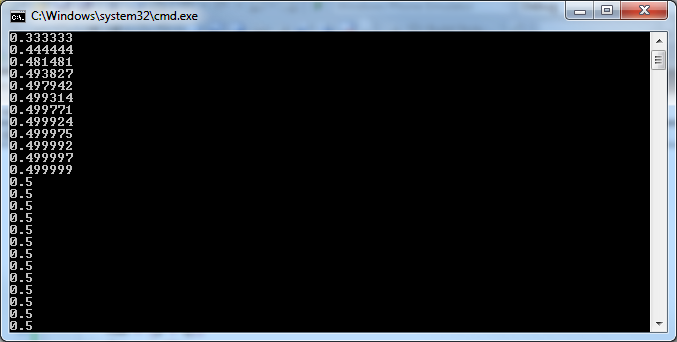
\includegraphics[scale=0.5]{hw3.png} \text{ } \\

	As we can see, it converges to $\dfrac{1}{2}$ quite fast which is consistent with our limit result. Thus 
	the upper bound of $B$ is $\dfrac{1}{2}$. Next we will show that is also the least upper bound by contradiction. \\
	Suppose that there is another upper bound says $b$ that is $< \dfrac{1}{2}$, we exclude the "$=$" sign here because the least upper bound
	must be unique. Since $b$ is the least upper bound of $B$, we have that for all $b_n \in B, n = 0, 1, 2, \ldots$, $b_n \leq b$, and this is clearly a contradiction
	because as we just have proved above, $b_n \rightarrow \dfrac{1}{2}$ as $n \rightarrow \infty$. Therefore the $\mathrm{sup}(B) = \dfrac{1}{2}$.
	\end{proof}
	\end{enumerate}
	
	\phantomsection
	\subsection*{{\color{purple}\underline{Problem 2}}}
	\addcontentsline{toc}{subsection}{\numberline{}Problem 2}
	Let $\mathbf{F}$ be an ordered field with the least upper bound property. Prove that if
	$a > 1$ is any number in $\mathbf{F}$, then the set $\{a, a^2, a^3, \ldots \}$ is not bounded above. 
	\begin{proof}
		We will prove this by contradiction. Suppose that $S = \{a, a^2, a^3, \ldots\}$ is bounded above, where $a \in \mathbf{F}$  and
		$\mathbf{F}$ is an ordered field with the least upper bound property. Now recall \textbf{ Theorem 4.2 } in lecture note 4:
		\newtheorem*{thm}{Theorem 4.2}
		\begin{thm}
			If $\mathbf{F}$ is an ordered field with the least upper bound property, then the following are true.
			\begin{enumerate}[(i)]
				\item The subset $\mathbf{N} \subset \mathbf{F}$ is not bounded above. 
				\item For each $a \in \mathbf{F_{+}}$, there is $n \in \mathbf{N}$ such that $\dfrac{1}{n} = n^{-1} < a$
				\item For each $a \in \mathbf{F}$, there is $m \in \mathbf{Z}$ such that $m \leq a \leq m + 1$ 
				\item For each $a \in \mathbf{F}$ and $\epsilon \in \mathbf{F_{+}}$, there is a rational number $r \in \mathbf{Q}$
				such that $|a - r| < \epsilon$		
			\end{enumerate}
		\end{thm}
		Hence, if $S$ is bounded above, then the least upper bound must exists. 
		Let's $b$ be the least upper bound of $S$, then all elements in $S$ is less than or equal to $b$ including all other
		upper bounds of $S$ of-course. In other words, $a^n \leq b, \, \, \forall n \in \mathbf{N}$. 
		On the other hand, $\mathbf{F}$ is an ordered field with the least upper bound property, 
		so $b \cdot a^{-1}$ is also an upper bound of $S$. This leads to the contradiction because we just claim that $b$
		is the least upper bound of $S$ or $\mathrm{sup(S)}$, but 
		$$ba^{-1} = \dfrac{b}{a} < b \, \, \text{ because } a > 1$$
		Therefore $S$ is not bounded above.
	\end{proof}
	
	\phantomsection
	\subsection*{{\color{purple}\underline{Problem 3}}}
	\addcontentsline{toc}{subsection}{\numberline{}Problem 3}
	Let $\mathbf{F}$ be an ordered field with the least upper bound property. Prove that for any number
	$a \in \mathbf{F}$ and any $\epsilon > 0$ there is natural number $n$ such that $\dfrac{a}{2^n} < \epsilon$. \\
	\begin{proof}
		We will prove this by contradiction. Suppose that $\exists a \in \mathbf{F}$ and $\exists \epsilon > 0$, for 
		all natural numbers $n$, then $\dfrac{a}{2^n} \geq \epsilon \Leftrightarrow 
		a \geq \epsilon \cdot 2^n$. However, $F$ is an ordered field with the least upper bound property which implies
		the largest lower bound as well. Look at the expression:
		$$a \geq \epsilon \cdot 2^n$$
		which tells us that $\epsilon \cdot 2^n, \forall n \in \mathbf{N}$ is clearly a lower bound of $a$, which implies
		there exists the largest lower bound. But we can increase $n$ forever, to obtain a larger and larger lower bound which 
		contradicts there exists the largest lower bound. Therefore for any number
		$a \in \mathbf{F}$ and any $\epsilon > 0$ there is natural number $n$ such that $\dfrac{a}{2^n} < \epsilon$
	\end{proof}
	
	
	\phantomsection
	\subsection*{{\color{purple}\underline{Problem 4}}}
	\addcontentsline{toc}{subsection}{\numberline{}Problem 4} \text{  } 
	\begin{enumerate}[(i)]
		\item Prove that $$\mathrm{max\{a, b\}} = \dfrac{a + b + |b - a|}{2}$$
		\item Derive a similar formula for $\mathrm{max\{a, b, c\}}$ using for example,
		$\mathrm{max\{a, b, c\}} = \mathrm{max}\{a, \mathrm{max\{b, c\}}\}$
	\end{enumerate}
	\begin{enumerate}[(i)]
		\item To prove this formula, we just need to break it into three cases.
		\begin{proof}
			If $b > a \Rightarrow |b - a| = b - a$, then
			$$\dfrac{a + b + |b - a|}{2} = \dfrac{a + b + b - a}{2} = \dfrac{2b}{2} = b$$
			If $a < b \Rightarrow |b - a| = -(b - a) = a - b$, then 
			$$\dfrac{a + b + |b - a|}{2} = \dfrac{a + b + a - b}{2} = \dfrac{2a}{2} = a$$
			If $a = b$ then 
			$$\dfrac{a + b + 0}{2} = \dfrac{2a}{2} = \dfrac{2b}{2} = a = b$$
			Thus $$\mathrm{max\{a, b\}} = \dfrac{a + b + |b - a|}{2}$$
		\end{proof}
		\item Using the given formula for two numbers we can derive the max of three numbers as follows:
		\begin{eqnarray*}
			\mathrm{max\{a, b, c\}} & = & \mathrm{max}\{a, \mathrm{max\{b, c\}}\} \\
			 & = & \dfrac{a + \mathrm{max}\{b, c\} + |\mathrm{max}\{b, c\} - a|}{2} \\
			 & = & \dfrac{a + \dfrac{b + c + |c - b|}{2} + \bigg|\dfrac{b + c + |c - b|}{2} - a\bigg|}{2} \\
			 & = & \dfrac{\dfrac{2a + b + c + |c - b|}{2} + \bigg|\dfrac{b + c + |c - b| - 2a}{2}\bigg|}{2} \\
		\end{eqnarray*}
	\end{enumerate}
	
	\phantomsection
	\subsection*{{\color{purple}\underline{Problem 5}}}
	\addcontentsline{toc}{subsection}{\numberline{}Problem 5}
	Prove that if 
	$$|x - x_0| < \dfrac{\epsilon}{2} \text{ and } |y - y_0| < \dfrac{\epsilon}{2}$$
	then 
	$$|(x + y) - (x_0 + y_0)| < \epsilon \text{ and } |(x - y) - (x_0 - y_0)| < \epsilon$$
	\begin{proof}
		Since $|x - x_0| \geq 0$ and $|y - y_0| \geq 0$, we have:
	$$|x - x_0| + |y - y_0| < \dfrac{\epsilon}{2} + \dfrac{\epsilon}{2} = \epsilon$$
	Now consider
		$$|(x + y) - (x_0 + y_0)| = |(x - x_0) + (y - y_0)| = |x - x_0| + |y - y_0| < \epsilon$$
	and 
		$$|(x - y) - (x_0 - y_0)| = |(x - x_0) + (y_0 - y)| = |x - x_0| + |y_0 - y| 
		= |x - x_0| + |y - y_0| < \epsilon$$	 
	\end{proof}		
	
	\phantomsection
	\subsection*{{\color{purple}\underline{Problem 6}}}
	\addcontentsline{toc}{subsection}{\numberline{}Problem 6}
	Prove that if 
	$$|x - x_0| < \dfrac{\epsilon}{2(|y_0| + 1)} \text{ and } |x - x_0| < 1 \text{ and }
	|y - y_0| < \dfrac{\epsilon}{2(|x_0| + 1)}$$
	then $$|xy - x_0y_0| < \epsilon$$
	(Hint. Write $xy - x_0y_0$ in a way that involves $x - x_0$ and $y - y_0$) 
	\begin{proof}
	We have that:
	\begin{eqnarray*}
		|xy - x_0y_0| &=& |(xy - xy_0 + xy_0 - x_0y_0)| \\
		&=& |x(y - y_0) + y_0(x - x_0)| \\
		&\leq& |x(y - y_0)| + |y_0(x - x_0)| \text{ by triangle inequality }\\
		&=& |x| \cdot |y - y_0| + |y_0| \cdot |x - x_0| \\
		&<& |x| \dfrac{\epsilon}{2(|x_0| + 1)} +  |y_0| \cdot \dfrac{\epsilon}{2(|y_0| + 1)}\\
		&=& \dfrac{\epsilon}{2} \cdot \dfrac{|x|}{|x_0| + 1} +  \dfrac{\epsilon}{2} \cdot \dfrac{|y_0|}{|y_0| + 1}\\
	\end{eqnarray*}
	Now what we need to show is 
	$$\dfrac{|x|}{|x_0| + 1} \leq 1 \text{ and } \dfrac{|y_0|}{|y_0| + 1} \leq 1$$
	and we're done. \\
	The second one is trivial since $\dfrac{|y_0|}{|y_0| + 1} \leq 1
	\Leftrightarrow |y_0| \leq |y_0| + 1 \Leftrightarrow 0 \leq 1$ which is true. To show the first inequality is true, we need
	$|x - x_0| < 1$ from the hypothesis which is equivalent to:
	$$-1 < x - x_0 < 1 \Rightarrow x < x_0 + 1$$
	Thus,
	$$|xy - x_0y_0| < \dfrac{\epsilon}{2} \cdot \dfrac{|x|}{|x_0| + 1} +  \dfrac{\epsilon}{2} \cdot \dfrac{|y_0|}{|y_0| + 1} < 
	\dfrac{\epsilon}{2} + \dfrac{\epsilon}{2} = \epsilon$$
	\end{proof}
	
	\phantomsection
	\subsection*{{\color{purple}\underline{Problem 7}}}
	\addcontentsline{toc}{subsection}{\numberline{}Problem 7}
	Prove that if $x_0 \neq 0$ and 
	$$|x - x_0| < \mathrm{min}\bigg\{\dfrac{|x_0|}{2}, \dfrac{\epsilon|x_0|^2}{2} \bigg\}$$
	then $x \neq 0$ and $\bigg|\dfrac{1}{x} - \dfrac{1}{x_0}\bigg| < \epsilon$ 
	\begin{proof}
	We have that,
	$$
	M = \mathrm{min}\bigg\{\dfrac{|x_0|}{2}, \dfrac{\epsilon|x_0|^2}{2} \bigg\} = 	
	\begin{cases} 
		\dfrac{|x_0|}{2} &, \text{ if } \dfrac{|x_0|}{2} < \dfrac{\epsilon|x_0|^2}{2} \, \, (1) \\
		\dfrac{\epsilon|x_0|^2}{2} &, \text{ if } \dfrac{|x_0|}{2} > \dfrac{\epsilon|x_0|^2}{2} \, \, (2) \\
	\end{cases}
	$$
	If $M = \dfrac{|x_0|}{2} \Rightarrow |x - x_0| < \dfrac{|x_0|}{2} \Rightarrow
	x \neq 0$ otherwise $|x_0| < \dfrac{|x_0|}{2}$ is nonsense because $x_0 \neq 0$. \\
	If $M = \dfrac{\epsilon|x_0|^2}{2} \Rightarrow |x - x_0| < \dfrac{\epsilon|x_0|^2}{2}
	\Rightarrow x \neq 0$ otherwise
	$\Rightarrow |x_0| <  \dfrac{\epsilon|x_0|^2}{2}$ is also nonsense because $x_0 \neq 0$ \\
	On the other hand, we have
	$$\bigg|\dfrac{1}{x} - \dfrac{1}{x_0}\bigg| =
	\bigg|\dfrac{x_0 - x}{xx_0}\bigg|
	$$
	Now we are ready to prove the other part by considering two cases:
	\begin{itemize}
		\item (1) $|x - x_0| < \dfrac{|x_0|}{2} < \dfrac{\epsilon|x_0|^2}{2}$ \\
		From $|x - x_0| < \dfrac{\epsilon|x_0|^2}{2} \Rightarrow \epsilon
		> \dfrac{2|x - x_0|}{|x_0|^2} > \bigg|\dfrac{x_0 - x}{xx_0}\bigg| = \bigg|\dfrac{1}{x} - \dfrac{1}{x_0}\bigg|$
		\item (2) $|x - x_0| < \dfrac{\epsilon|x_0|^2}{2} < \dfrac{|x_0|}{2}$ \\
		From $|x - x_0| < \dfrac{\epsilon|x_0|^2}{2} \Rightarrow
		\epsilon > \dfrac{2|x - x_0|}{|x_0|^2} > \bigg|\dfrac{x_0 - x}{xx_0}\bigg| = \bigg|\dfrac{1}{x} - \dfrac{1}{x_0}\bigg|$
	\end{itemize}
	\end{proof}
	
	
	\phantomsection
	\subsection*{{\color{purple}\underline{Problem 8}}}
	\addcontentsline{toc}{subsection}{\numberline{}Problem 8}
	Let $\mathbf{F}$ be an ordered field with the least upper bound property. If $A \neq \emptyset$ is bounded below,
	let $B$ be the set of all lower bounds of $A$. Prove that:
	\begin{enumerate}[(i)]
		\item $B \neq \emptyset$
		\item $B$ is bounded above 
		\item $\mathrm{sup}(B) = \mathrm{inf}(A)$
	\end{enumerate}
	\begin{proof}
	The set $B \neq \emptyset$ because $A$ is bounded below (any lower bound for $A$ is in $B$).
	Because $A$ is nonempty, there is $a$ in $A$, and this $a$ satisfies $y \leq a$ for all $y$ in $B$.
	Because of this, $y \leq x$ for all $x$ in $A$ and all $y$ in $B$, and thus $\sup(B) \leq \inf(A)$.
	If $\sup(B) < \inf(A)$, then there is a number $x$ such that $\sup(B) < x < \inf(A)$. The inequality
	$\sup(B) < x$ implies that $b < x$ for all $b \in B$ and thus that $x$ is not in $B$. The inequality
	$x < \inf(A)$ implies that $x < a$ for all $a$ in $A$, and thus that $x$ is a lower bound for $A$.
	Therefore $x$ is in $B$. But this contradicts the inequality $\sup(B) < x$ as noted.
	\end{proof}
	
	
	\phantomsection
	\subsection*{{\color{purple}\underline{Problem 9}}}
	\addcontentsline{toc}{subsection}{\numberline{}Problem 9}
	Let $\mathbf{F}$ be an ordered field with the least upper bound property. Let $A \subset \mathbf{F}$ be a
	nonempty set of numbers. Prove that $\alpha = \mathrm{sup}(A)$ if and only if $\alpha$ is an upper bound for $A$
	and for any $\epsilon > 0$, there is an $x$ in $A$ such that $\alpha < x + \epsilon$. 
	\begin{proof} To prove if and only if, we need to prove it for both direction, and we will
		prove this by contradiction.
		\begin{itemize}
			\item $\Rightarrow:$ The contradiction can be written as follows: \\ 
			If $\alpha = \mathrm{sup}(A)$ then $\alpha$ is an upper bound for $A$
			and $(\exists \epsilon > 0)(\forall x \in A)$ such that $\alpha \geq x + \epsilon$.
			Note that we don't take the part $\alpha$ is an upper bound for $A$ into the statement, and 
			apply Demorgan's law: $\neg(A \text{ and } B) = \neg(A) \text{ or } \neg(B)$ strictly because
			it's trivially true when $\alpha = \mathrm{sup}(A)$. On the other hand, this supposition implies
			that $\alpha - \epsilon$ is also the least upper bound of $A$ because $\alpha - \epsilon \geq x, \, \, \forall x \in A$. Furthermore $\epsilon > 0$ and
			$\alpha - \epsilon < \alpha$, this is a contradiction. Therefore if $\alpha = \mathrm{sup}(A)$ then 
			$\alpha$ is an upper bound for $A$ and for any $\epsilon > 0$, there is an $x$ in $A$ 
			such that $\alpha < x + \epsilon$.
			
			\item $\Leftarrow:$ To prove from this side, we assume that if $\alpha$ is an upper bound for $A$
			and for any $\epsilon > 0$, there is an $x$ in $A$ such that $\alpha < x + \epsilon$ then $\alpha \neq
			\mathrm{sup}(A)$.
			This side is too obvious and it leads to contradiction immediately.  
		\end{itemize}
	\end{proof}

	\phantomsection
	\subsection*{{\color{purple}\underline{Problem 10}}}
	\addcontentsline{toc}{subsection}{\numberline{}Problem 10}
	Let $\mathbf{F}$ be an ordered field with the least upper bound property. Let $A \subset \mathbf{F}$ and 
	$B \subset \mathbf{F}$ be the two nonempty sets of numbers that are bounded above, and let $A + B$ denote the set
	of all numbers of the form $x + y$ with $x \in A$ and $y \in B$. 
	Prove that $\mathrm{sup}(A + B) = \mathrm{sup}(A) + \mathrm{sup}(B)$. 
	\begin{proof}
	Since $x \leq \sup(A)$ and $y \leq \sup(B)$ for every $x$ in $A$ and $y$ in $B$, it follows that
	$x + y \leq \sup(A) + \sup(B)$. Thus $\sup(A) + \sup(B)$ is an upper bound for $A + B$, so 
	$\sup(A + B) \leq \sup(A) + \sup(B)$. If $x$ and $y$ are chosen in $A$ and $B$, respectively,
	so that $\sup(A) - x < \epsilon/2$ and $\sup(B) - y < \epsilon/2$, then $\sup(A) + \sup(B) - (x + y) < \epsilon$.
	Hence $\sup(A + B) \geq x + y > \sup(A) + \sup(B) - \epsilon$.
	\end{proof}	 
	
	\phantomsection
	\subsection*{{\color{purple}\underline{Problem 11}}}
	\addcontentsline{toc}{subsection}{\numberline{}Problem 11}
	Suppose that $A$ and $B$ are 2 non-empty sets of numbers such that $x \leq y$ for all $x$
	in $A$ and all $y$ in $B$.
	\begin{enumerate}[(a)]
		\item Prove that $\sup(A) \leq y$ for all $y \in B$.
		\begin{proof}
			Since any $y$ in $B$ satisfies $y \geq x$ for all $x$ in $A$, any $y$ in $B$ is an upper bound
			for $A$, so $y \geq \sup(A)$.
		\end{proof}
		\item Prove that $\sup(A) \leq \inf(B)$
		\begin{proof}
			Part (a) shows that $\sup(A)$ is a lower bound for $B$, so $\sup(A) \leq \inf(B)$.
		\end{proof}
	\end{enumerate}
\end{document}
